\documentclass[titlepage]{article}   	% use "amsart" instead of "article" for AMSLaTeX format
\usepackage{geometry}                		% See geometry.pdf to learn the layout options. There are lots.
\geometry{letterpaper}                   		% ... or a4paper or a5paper or ... 
%\geometry{landscape}                		% Activate for rotated page geometry
%\usepackage[parfill]{parskip}    		% Activate to begin paragraphs with an empty line rather than an indent
\usepackage{graphicx}				% Use pdf, png, jpg, or eps§ with pdflatex; use eps in DVI mode
								% TeX will automatically convert eps --> pdf in pdflatex		
\usepackage{amssymb}
\usepackage{dcolumn}
\usepackage[capposition=top]{floatrow}
\usepackage{booktabs}
\usepackage{rotating,tabularx}

%SetFonts

%SetFonts


\title{Exploring the Factors Influencing Admission to an Elite University: A Random Forests Approach}
\author{David K. Kirui}
%\date{}							% Activate to display a given date or no date

\begin{document}
\maketitle
\section{Statement of the Problem}

College admissions are a stressful process for students, parents, and educators. Decisions handed down by undergraduate admissions committees can have profound impacts on students’ educational and career trajectories and, at a macro level, on the life course. Many professionals working in the field of guidance and educational counseling must strike a balance between accurately advising students of their admissions chances while not discouraging their post-secondary aspirations. As such, developing tools that can assist educational professionals in providing the best, most reliable advice to high school students applying to colleges is of crucial import. To that end, this report seeks to develop and refine a pilot algorithm which, in the future, may be used to aid our own internal college advising processes. Generally, this report draws upon tools of machine learning to evaluate what factors of students’ academic and demographic profiles are related to their admission to college. Although the data available on which to pilot this algorithm are fairly limited in scope, the hope is that we can begin to use similar algorithms on more robust and probabilistic data in the near future with the goal of enhancing the support we provide to our college-going students.

\section{Description of the Data}

The data used in this report are a dataset obtained from an unknown “elite” university and contain information about some of the applications they received in the prior year, including whether or not applicants were admitted. A third party collected these data and noted that they were neither a random probabilistic sample of applicants nor the total pool of applicants to that university in that year. As such, arguing that a level II analysis is warranted is difficult. Although random forests introduces randomness into the algorithm, this is not related to how the data were generated. The randomness necessary to generalize beyond the data on hand is simply not present, so this analysis cannot move beyond level I. \footnote{\label{myfootnote} Berk, Richard A. Statistical learning from a regression perspective. Vol. 14. New York: Springer, 2008. P. 210} 

Data collection yielded a total sample size of 8,700 observations. A dichotomous measure (admit) indicates whether or not an applicant was admitted. A dummy variable captures their biological sex. These data also include three dichotomous measures capturing applicants race/ethnicity (anglo, asian, and black). In addition, these data include a measure of applicants’ high school grade point averages (GPAs), weighted to account for Advanced Placement (AP) course taking (gpa.wtd). Data were also included that measured applicants’ scaled scores on the verbal and math sections of their SAT 1 (sat1.verb and sat1.math respectively). Lastly, a measure of applicants’ household income was included (income); it can be reasonably assumed that this is an annual measure, although it’s not explicitly clear. In total, these data included nine raw variables. Because these data were not generated in such a way that they are a random probabilistic sample, the data do not strictly allow us to move beyond level I analysis. It follows, therefore, that we cannot generalize to the larger applicant pool of this university in this or any given year, or to universities with similar applicant profiles. 

\section{Cleaning up the Data}

These data have a total of 8,700 observations. The only variable for which the data were completely intact was the variable that measured admission. All of the other 8 variables had information that was either missing or problematic in some other way. 19.8\% of cases had missing information on household income. 9.5\% of cases were missing information on the variable that measured whether or not applicants were White (anglo). There were also about 10\% of cases that had missing information on the variables that measured whether or not someone was Asian (asian) or Black (black). Less than 1\% (.27\%) of data were missing on the variable that measured applicants’ biological sex. Missing cases on these variables were all treated via list-wise deletion. 

In addition to the missing cases noted above, there were also a number of observations on variables that were implausible. 19 observations had weighted GPAs recorded as zero; this accounted for .2\% of the sample. 5.2\% of applicants had SAT1 math and verbal scores of 0; this is not possible since the lowest score one could attain on either section is 200. There were also a number of very low values for household income (5 values below \$1,000). Although it is improbable that applicants would have household incomes this low, it is possible and, therefore, I decided to keep these values in the dataset. Moreover, there were very few of these observations so they wouldn’t affect the distribution of income. Observations that were implausible and could not be modified were treated as true missing values and dropped via list-wise deletion. In total, 29\% of cases had missing data on at least one observation and were dropped; this reduced the sample size to 6,175 observations, all of which were complete cases. 
 
Next, I created a new variable for race, creating one categorical measure with four possible categories: 1) White, 2) Asian, 3) Black, and 4) Other. Categorizing race in this way highlighted the fact that there are individuals in the dataset who are not White, Asian, or Black. I then performed a linear basis expansion on weighted GPA, taking its square.\footnote{\label{myfootnote} I also took the log and square of income, but it had no impact on its distribution.} This transformation was done to better accommodate possible non-linearity in GPA and make its distribution more normal while preserving the linear functional form. The R code that I used to clean the data and conduct all of the analyses presented in this report are available in an appendix.

\section{Analysis of Univariate Statistics}

Descriptive statistics for each variable in the full dataset can be found in Table 1. I also tabulated descriptive statistics on the test subset (omitted) and the results closely approximated those found in Table 1. Histograms depicting the distributions of continuous measures can be found in Figure 1. On average, applicants had weighted GPAs of 3.81 and median weighted GPAs of 3.86, indicating that the distribution is somewhat left-skewed (see Figure 1). At minimum, applicants had weighted GPAs of 1.25 and at maximum they had weighted GPAs of 4.95, with a standard deviation of about .48.  The mean SAT1 Verbal Score was about 578, while the median score was 580. The minimum verbal score was 200 while the maximum was 800. The standard deviation of verbal scores was just over 100. Like weighted GPA, the distribution of SAT verbal scores was also slightly left skewed (see Figure 1). On average, applicants scored about 620 on the SAT 1 math, with a median score of 630. The minimum SAT 1 Math score was 220, the maximum score was 800, with a standard deviation of 98.47. Like weighted GPA and SAT1 Verbal, SAT1 Math scores were also slightly left-skewed (see Figure 1). The left-skewed nature of these variables suggests that the applicant pool represented here had above average academic achievement. 

The average household income among applicants was \$62,944, while the median household income was \$65,000. At minimum, applicants’ household income was \$120; at maximum, it was \$99,999 with a standard deviation of \$32,790.59. As mentioned when data cleaning was discussed, while household incomes as low as \$120 are improbable, they were kept in the dataset because they are possible. Moreover, there are very few observations on the low end, so the practical impact of these observations on the distribution is low. Likewise, it is important to note that the dataset was truncated at \$99,999. As illustrated in Figure 1, the distribution for income is heavily left skewed, with a plurality of observations clustered at or just below \$99,999. This suggests that had the data not been truncated, there may be a significant number of observations at or above \$100,000. Less than 1 out of 3 (31.17\%) applicants were admitted. 45.55\% of applicants were male. A plurality of applicants identified as Asian or Asian-American (45.43\%), 33.33\% of applicants identified as White, 4.31\% of applicants as Black or African-American, and 16.93\% of applicants as belonging to some other race. 

\section{Analysis of Bivariate Statistics}

To analyze the relationship between our response variable, admit, and each of our predictors, I generated a series of bivariate boxplots (see Figure 2) and contingency tables (see Table 2). In addition, I generated pairwise scatterplots with loess smoothers to analyze the relationships among the continuous predictors (see Figure 3). First, we can see by looking at the boxplot of weighted GPA by admission, that although admitted applicants have higher median, 75th, and 25th percentile GPAs than their peers that were rejected, there is greater variability in GPA among rejected applicants. Moreover, rejected applicants have both higher maximum and minimum GPAs than their accepted peers. When looking at the boxplots that parse admittance by SAT1 verbal and math test scores, we can see similar trends. In each case, the interquartile ranges lie higher on the spectrum of possible scores, but the ranges of scores for admitted students are more narrow than for their rejected peers. Like GPA, there are some rejected students who had test scores that were at or near perfect. Though this may seem counterintuitive, there is a body of literature that suggests that selective schools, when faced with many applicants with stellar grades and test scores, opt for more well rounded students over their counterparts with perfect academic records but deficiencies elsewhere. \footnote{\label{myfootnote} Sternberg, R. J. (2010). College admissions for the 21st century. Harvard University Press.} 

The relationship between admission and household income is the most idiosyncratic in the dataset, likely because these data were truncated to have an upper bound of \$99,999. Both rejected and admitted applicants span the entire range of possible income values, though the median and 25th percentile for income are higher for admitted applicants than their rejected peers. The 75th percentile for both classes of applicants appears to be at or near the maximum possible value of \$99,999. When looking at the relationship between admission and sex (see Table 2), we see that a slightly lower percentage of male applicants (30\%) are admitted than their female peers (32\%). Likewise, we can see from Table 2 that among racial groups,  33\% of White applicants were admitted, followed closely by 32\% of their Asian peers; somewhat lower percentages of Black applicants (27\%) and applicants that identified as belonging to another racial group (26\%) were admitted. When analyzing the relationship between the continuous predictors (see Figure 3), it appears that a positive linear relationship exists among each of the measures of academic achievement (Weighted GPA, SAT1 Verbal, and SAT1 Math respectively). Moreover, it appears that there is also a positive relationship between income and each measure of academic achievement, although income appears to have a weaker impact on GPA than on test score (as evidenced by the more shallow loess smoother). 

\section{Random Forests Analysis}

First, I constructed two datasets of equal size: a training dataset, and a test dataset. I subsequently used the training dataset to train the random forest algorithm until I was able to find a cost ratio that approximated my target cost ratio. After arriving at an algorithm that approximated my ideal cost ratio, I ran the random forest algorithm in the test data to generate a final analysis forest from which I derived a final confusion table and my final algorithmic forecasts. To accomplish this, I used the randomForest package in R and kept the default settings, growing 500 trees within each forest. For this analysis, I decided that my ideal cost ratio was 4 to 1. I arrived at this cost ratio because there is a robust body of literature \footnote{\label{myfootnote} Avery, C. (2010). The effects of college counseling on high-achieving, low-income students (No. w16359). National Bureau of Economic Research.; Hoxby, C. M., Avery, C. (2012). The Missing" One-Offs": The Hidden Supply of High-Achieving, Low Income Students (No. w18586). National Bureau of Economic Research.} in higher education that suggests that prospective college students, particularly from high achieving low-income backgrounds, may not apply to selective colleges for which they are competitive. By this rationale, I decided that it is 4 times as costly to wrongly advise a student that they would be rejected (false negative) than to wrongly advise a student that they’d be accepted (false positive). While a false positive, in this case, would at most result in a bruised ego, a false negative could potentially result in a missed opportunity that could have profound implications on the life course. 

Once I decided upon the target cost ratio, I grew a series of random forests in the training data each time iterating the prior distribution (base rate) to capture the cost ratio as each tree was grown. I started with a sample size of 623 for the admitted class, which equaled 2/3 the number of cases in that class. \footnote{\label{myfootnote} I calculated this starting value based on training data.} Based on the 50-50 constraint, I began with a sample size of 623 in the reject class as well. After growing the first forest, I grew 5 additional forests, tuning the base rate each time to arrive at a cost ratio that closely approximated my target. Diagnostic information for each of the six forests that I used for tuning purposes can be found in Table 3. On the sixth iteration of this process, I arrived at a forest that adequately approximated my target cost ratio with a base rate of 300 to 623 (Labeled RF 6 in Table 3).
After arriving at the final forest in the training data, I used the test data to grow this forest, gauge its performance, and interpret its results. The confusion table generated from this forest can be found in Table 4. From the table, we can see that the final forest yielded a use error rate for negative prediction (rejection) of .07 and an error rate for positive prediction (admittance) of .39. Put differently, the algorithm is right 93\% of the time when it forecasts that an applicant will be rejected. Moreover, the algorithm is right just 61\% of the time when it forecasts that an applicant will be admitted. Given how we assigned our cost ratio, it is not surprising that the resulting algorithmic forecast is very accurate when forecasting rejection. This forest also yielded a model error for rejection that is .27, a model error for acceptance of .11, and an overall error rate of .25. In other words, given that an applicant was rejected, the model correctly forecast it 73\% of the time and given that an applicant was admitted, the model correctly forecast it 89\% of the time. 

Next, I generated a series of plots to assess the contribution of each predictor to the overall “prediction accuracy" of the algorithm (e.g., classification accuracy in the out of bag (OOB) data) for both class outcomes. Figure 4 displays the unstandardized predictor importance plots for admittance and rejection, with the unstandardized reductions in prediction accuracy on the horizontal axes. Standardized plots are omitted. Each predictor is randomly shuffled in turn to arrive at these benchmarks. We can see that when forecasting both admission and rejection, GPA contributes the most to prediction accuracy. When GPA is randomly shuffled, the accuracy of the algorithm in predicting admission is reduced by 25\% and is reduced by about 5\% when predicting rejection. When predicting admission, SAT verbal and math scores also make substantial contributions. When SAT Verbal score is randomly shuffled, prediction accuracy is reduced by 10\%; when SAT Math score is shuffled, prediction accuracy is reduced by about 6\%. When forecasting admission, income, race, and sex, all contribute between about 3\% and about 0\% accuracy. When forecasting rejection, all predictors besides GPA make modest contributions to prediction accuracy, with each predictor contributing less than 2\% to prediction accuracy.

After gauging variable importance, I used partial dependence plots to gauge the direction of the relationship between each of my predictors and admissions decision holding all other predictors constant. Partial dependence plots for each of the predictors can be found in Figures 5 through 9, in order of importance.  Figure 5 shows the partial dependence plot for Weighted GPA (in squared units); From the upper plot, we see that the largest centered logit, for a student with about a 4.0, is about .5, while the smallest, for a student with about a 3.0 or less is about -.5. From the lower plot, we can see this difference in proportion units. These logits become proportions of about .80 and .20 respectively; the proportion of applicants who are admitted increases four-fold as GPA increases from 3.0 to 4.0. Figure 6 shows the partial dependence plots for SAT Verbal scores. We see here that the largest centered logit is above .4 and the smallest is below -.6; these logits become proportions greater than .7 and less than .3 respectively. The proportion of admitted applicants more than doubles as SAT verbal scores increase. Figure 7 shows the plots for SAT math scores. The largest centered logit here is slightly above .4 while the smallest is below -.2; these become proportions of .7 and less than .4. The proportion of admitted applicants increases a little less than two-fold as SAT math scores increase from 400 to 800. Figure 8 shows the plots for income; they suggest a modest decrease in the proportion of applicants accepted as incomes increase. The largest centered logit is slightly less than .20 while the smallest is about -.5; these become proportions of just shy of .60 and less than .50. The proportion of applicants that are admitted decreases by about .10 as incomes increase from 0 to 100,000, but it should be noted that there are relatively few very small observations and that the income variable was artificially truncated at \$100,000, leaving a good number of observations at the high end.

Lastly, Figure 9 shows plots for both sex and race. Here, female applicants are more likely to be admitted (with a centered logit about .03), while male applicants are less likely to be admitted (with a centered logit of less than -.01). The proportion of female applicants accepted is roughly .52 while the proportion of their male peers accepted is about .50, with a difference in proportion of about .02. The centered logit for Black applicants is about .15, applicants of another race is about .10, White applicants is about -.01, and Asian applicants about -.012. The proportion of Black applicants admitted is about .57, while the proportion of applicants of another race admitted is .55, White and Asian applicants both have proportions of admittance of about .49, with a difference in proportion between Black and White/Asian applicants of about .08. As evinced in the importance plot for admission, however, neither sex nor race adds much prediction accuracy to the algorithm. Important to note here is that the magnitude of the effects found in the partial dependence plots decrease in the order of their importance to prediction accuracy.

\section{Summary and Conclusions}

In sum, my analyses suggest that, for these data, the single most important factor in forecasting admittance to this university last year was an applicant’s weighted GPA. Applicants with higher weighted GPAs were more likely to gain admission. Applicants SAT1 scores on both the verbal and math sections also had a notable impact on forecasting admittance. SAT verbal performance seemed to have slightly more import than mathematics performance. In both cases, applicants with higher standardized test scores were more likely to gain admission. By contrast, applicants’ household income, race/ethnicity, and biological sex seemed to have little bearing on forecasting admission. Moreover, the algorithm does a stellar job at correctly classifying applicants who are rejected. When it forecasts that an applicant will be rejected, it is correct 93\% of the time. Since we determined that incorrectly advising an applicant that they will be rejected is more costly than incorrectly advising an applicant that they will be accepted, it makes sense that the algorithm works to minimize the number of false negatives.
 
It is clear that the admissions office at this university takes academic performance and past achievement heavily into account when making admissions decisions. Although these data give us insight into the particular subset of last year's applicant pool at that elite university, since they are neither a probabilistic sample from the applicant pool nor a sample of the entire applicant pool, justification to move beyond a level I analysis would be tenuous at best. Nonetheless, this analysis can provide us with insight into the admissions process for this particular subset of the applicant pool, at this university, at this particular point in time. Moreover, as we move forward in piloting this algorithm, these data have provided us with a useful baseline from which to continue to develop our algorithm to best serve our students. 


% Please add the following required packages to your document preamble:
% \usepackage{booktabs}
\begin{table}[]
\centering
\caption{Descriptive Statistics (Full Dataset)}
\label{my-label}
\begin{tabular}{@{}rl@{}}
\toprule
\multicolumn{1}{l}{}                             &          \\ \midrule
\multicolumn{1}{l}{\textbf{Weighted GPA}}        &          \\
Min.                                             & 1.25     \\
Max.                                             & 4.95     \\
Mean                                             & 3.808    \\
Median                                           & 3.86     \\
S.D.                                             & 0.48     \\
\multicolumn{1}{l}{\textbf{SAT 1 Verbal}}        &          \\
Min.                                             & 200      \\
Max.                                             & 800      \\
Mean                                             & 578.2    \\
Median                                           & 580      \\
S.D.                                             & 100.24   \\
\multicolumn{1}{l}{\textbf{SAT 1 Math}}          &          \\
Min.                                             & 220      \\
Max.                                             & 800      \\
Mean                                             & 619.5    \\
Median                                           & 630      \\
S.D.                                             & 98.47    \\
\multicolumn{1}{l}{\textbf{Income}}              &          \\
Min.                                             & 120      \\
Max.                                             & 99999    \\
Mean                                             & 62944    \\
Median                                           & 65000    \\
S.D.                                             & 32790.59 \\
\multicolumn{1}{l}{\textbf{Admitted (\%)}}       & 31.17    \\
\multicolumn{1}{l}{\textbf{Male (\%)}}           & 45.55    \\
\multicolumn{1}{l}{\textbf{Race/Ethnicity (\%)}} &          \\
White                                            & 33.33    \\
Asian                                            & 45.43    \\
Black                                            & 4.31     \\
Some Other Race                                  & 16.93    \\
\multicolumn{1}{l}{N}                            & 6175     \\ \bottomrule
\end{tabular}
\end{table}

\begin{figure} [h]
\centering
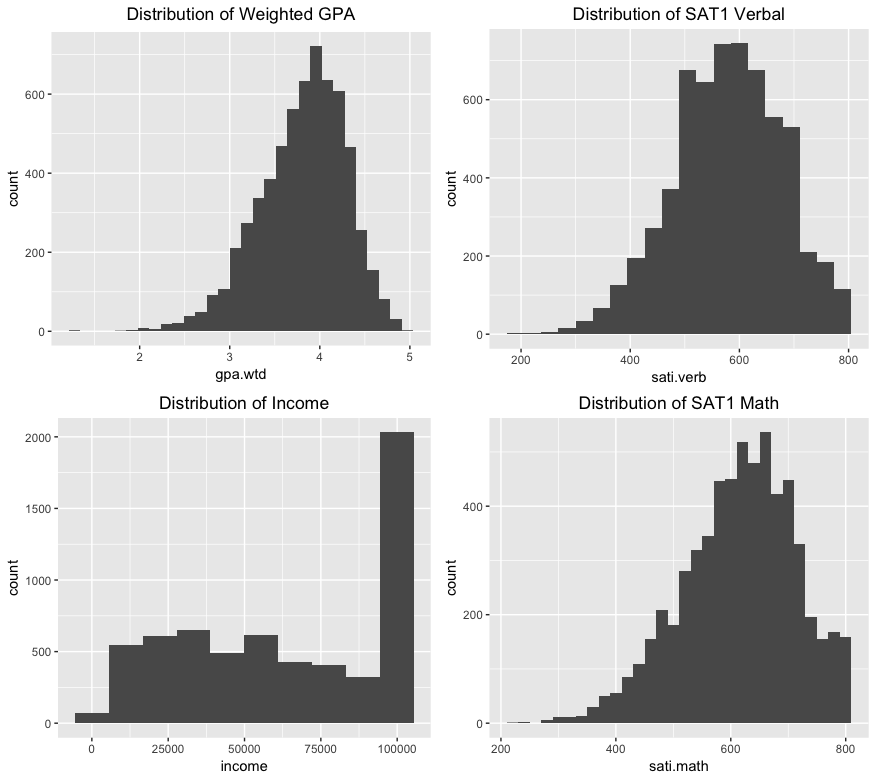
\includegraphics[scale=.50]{univariate}
\caption{Univariate Histograms for Continuous Measures (Full Dataset)}
\end{figure}

\begin{figure} [h]
\centering
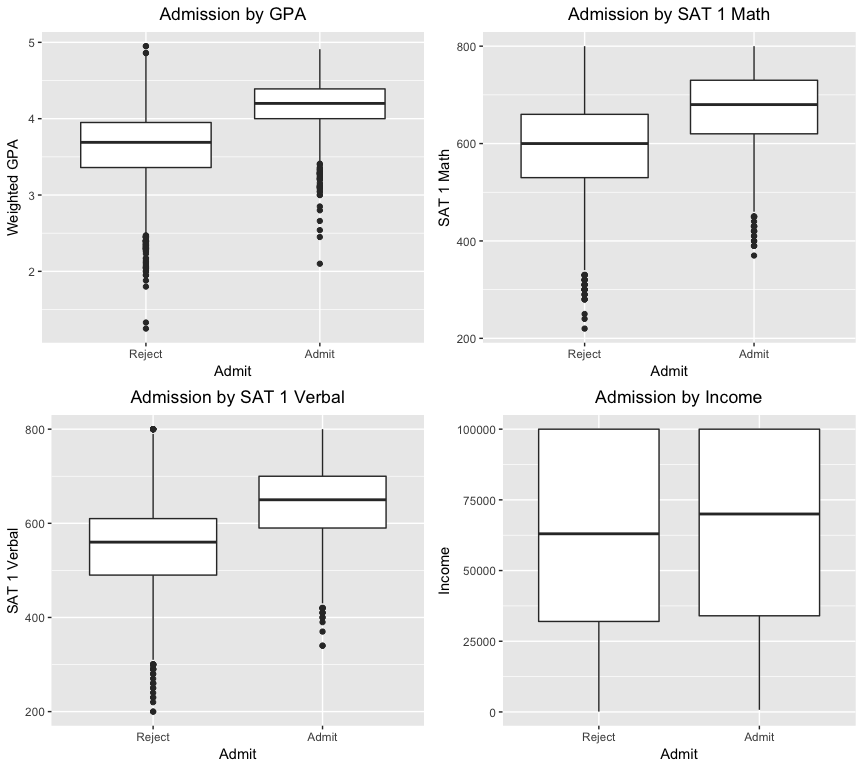
\includegraphics[scale=.50]{bivariate}
\caption{Bivariate Boxplots (Full Dataset)}
\end{figure}

\begin{figure} [h]
\centering
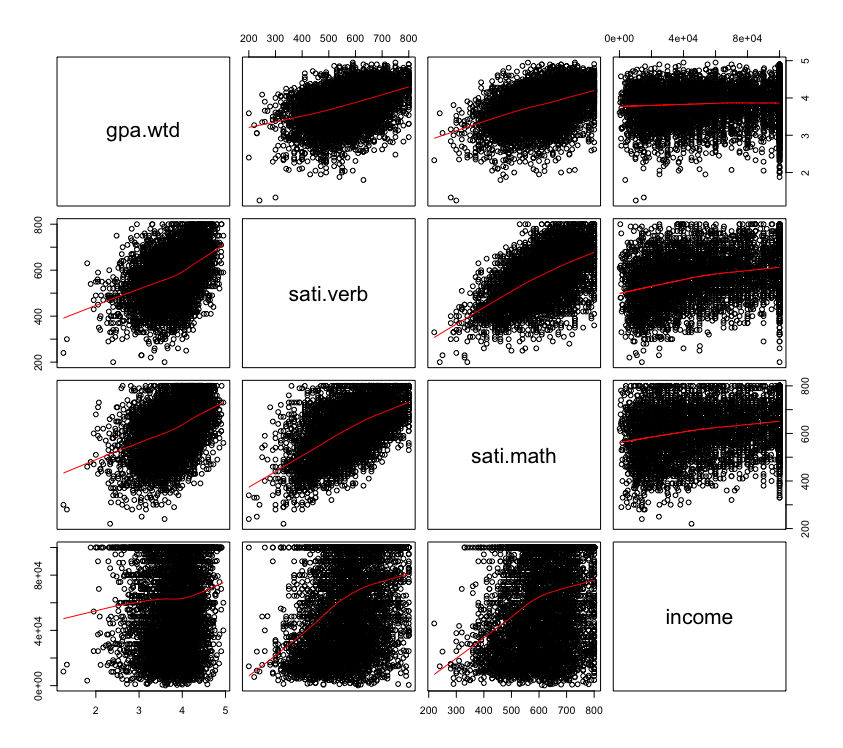
\includegraphics[scale=.50]{scatterplotmatrix}
\caption{Scatterplot Matrix of Continuous Predictors}
\end{figure}

% Please add the following required packages to your document preamble:
% \usepackage{booktabs}
\begin{table}[]
\centering
\caption{Contingency Tables for Categorical Predictors by Acceptance}
\label{my-label}
\begin{tabular}{@{}lllll@{}}
\toprule
\multicolumn{5}{c}{\textbf{Sex (\%)}}                                            \\ \midrule
                & \textbf{Reject} & \textbf{Admit} & \textbf{Total} & \textbf{n} \\
\textbf{Female} & 68              & 32             & 100            & 3362       \\
\textbf{Male}   & 70              & 30             & 100            & 2813       \\
\textbf{Total}  & 69              & 31             & 100            & 6175       \\ \midrule
\multicolumn{5}{c}{\textbf{Race/Ethnicity (\%)}}                                 \\ \midrule
\textbf{Other}  & 74              & 26             & 100            & 1046       \\
\textbf{White}  & 67              & 33             & 100            & 2058       \\
\textbf{Asian}  & 68              & 32             & 100            & 2805       \\
\textbf{Black}  & 73              & 27             & 100            & 266        \\
\textbf{Total}  & 69              & 31             & 100            & 6175       \\ 
\bottomrule
\end{tabular}
\end{table}









% Please add the following required packages to your document preamble:
% \usepackage{booktabs}
\begin{sidewaystable}[]
\centering
\caption{Algorithm Tuning Parameters}
\label{my-label}
\begin{tabular}{@{}lrrrrrrrr@{}}
\toprule
\textbf{RF} & \multicolumn{2}{c}{\textbf{Base Rate}} & \multicolumn{1}{l}{\textbf{Cost Ratio}} & \multicolumn{2}{c}{\textbf{Model Error}} & \multicolumn{2}{c}{\textbf{Use Error}} & \multicolumn{1}{l}{\textbf{Overall Error}} \\ \midrule
\textbf{} & \textbf{Reject} & \textbf{Admit} & \textbf{} & \textbf{Reject} & \textbf{Admit} & \textbf{Reject predicted} & \textbf{Admit predicted} & \textbf{} \\
1 & 623 & 623 & 2 to 1 & 0.158 & 0.216 & 0.100 & 0.318 & 0.184 \\
2 & 525 & 623 & 2 to 1 & 0.180 & 0.193 & 0.093 & 0.340 & 0.197 \\
3 & 400 & 623 & 3 to 1 & 0.212 & 0.160 & 0.081 & 0.368 & 0.218 \\
4 & 175 & 623 & 10 to 1 & 0.349 & 0.085 & 0.053 & 0.468 & 0.344 \\
5 & 275 & 623 & 5 to 1 & 0.272 & 0.123 & 0.068 & 0.417 & 0.267 \\
6 & 300 & 623 & 4 to 1 & 0.255 & 0.134 & 0.072 & 0.404 & 0.253 \\ \bottomrule
\end{tabular}
\end{sidewaystable}[]

% Please add the following required packages to your document preamble:
% \usepackage{booktabs}
\begin{table}[]
\centering
\caption{Final Confusion Matrix (Test Data)}
\label{my-label}
\begin{tabular}{@{}llll@{}}
\toprule
 & \textbf{Reject predicted} & \textbf{Admit predicted} & \textbf{Model error} \\ \midrule
\textbf{Reject} & 1537 & 560 & 0.27 \\
\textbf{Admit} & 109 & 882 & 0.11 \\
\textbf{Use error} & 0.07 & 0.39 & 0.25* \\ \bottomrule
\end{tabular}
\end{table}



\begin{figure} [h]
\centering
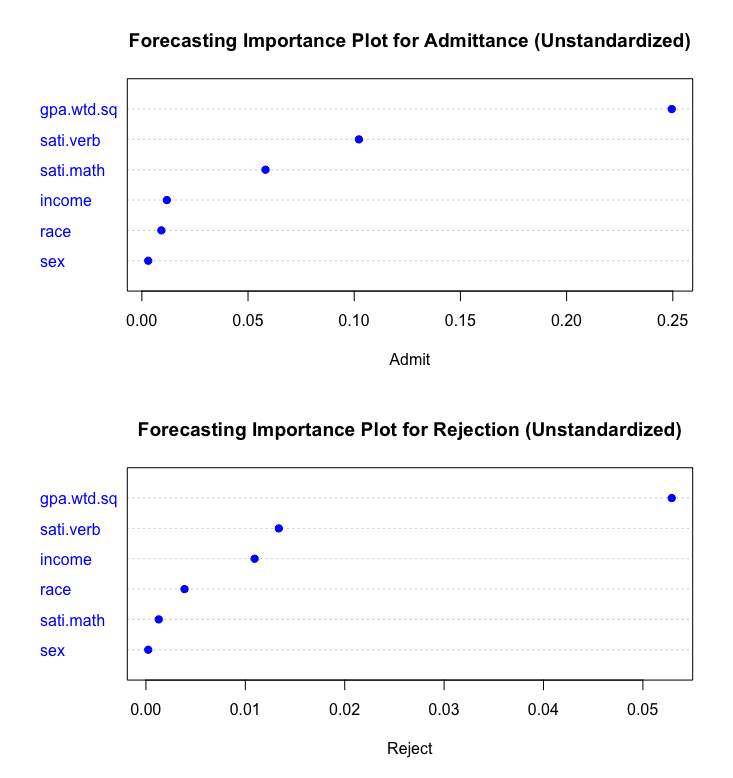
\includegraphics[scale=.60]{IMPORTANCE}
\caption{Importance Plots for Admittance (Test Data)}
\end{figure}

\begin{figure} [h]
\centering
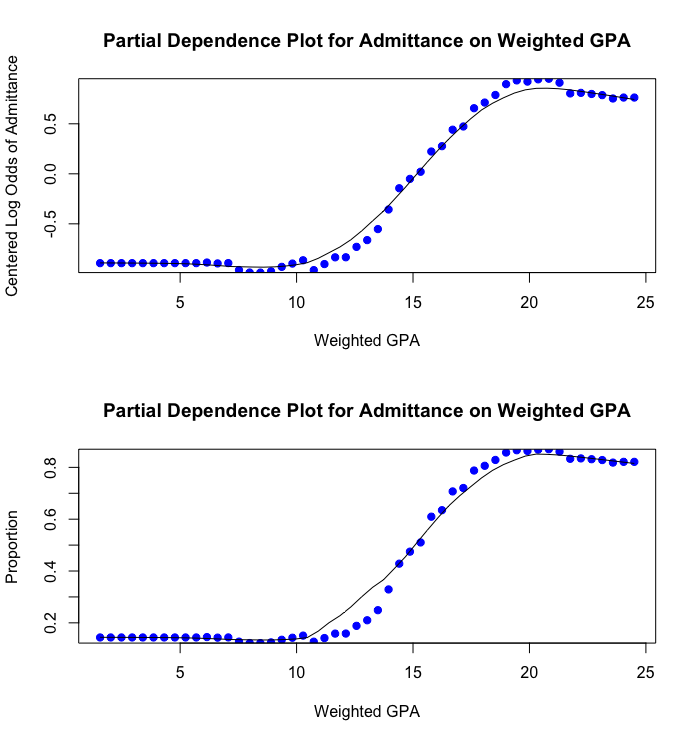
\includegraphics[scale=.60]{DEPENDENCE2}
\caption{Partial Dependence Plots for Weighted GPA (Sq.)}
\end{figure}

\begin{figure} [h]
\centering
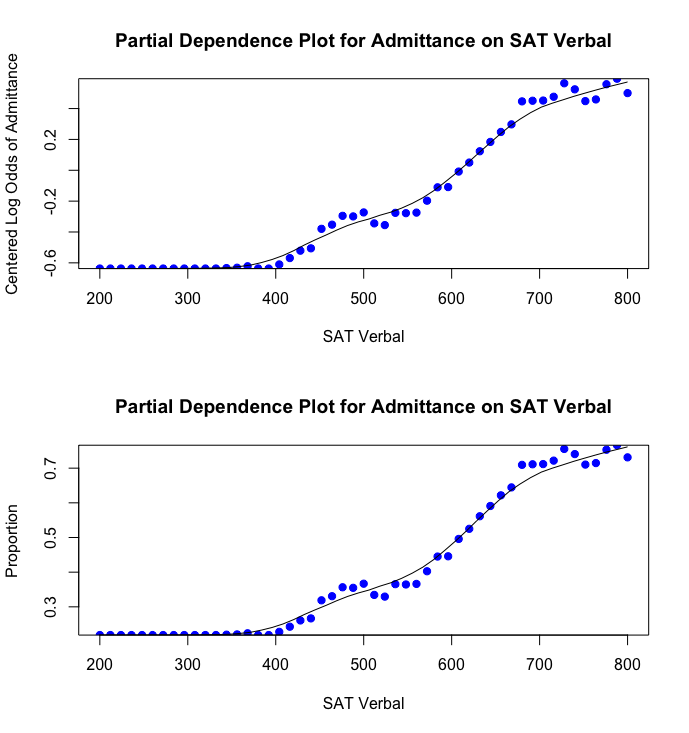
\includegraphics[scale=.60]{DEPENDENCE3}
\caption{Partial Dependence Plots for SAT Verbal Scores}
\end{figure}

\begin{figure} [h]
\centering
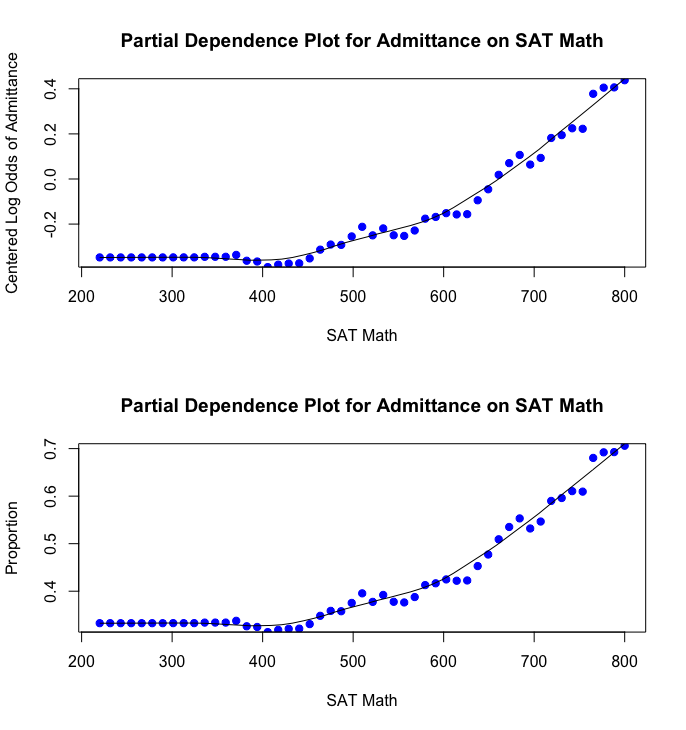
\includegraphics[scale=.60]{DEPENDENCE4}
\caption{Partial Dependence Plots for SAT Math Scores}
\end{figure}

\begin{figure} [h]
\centering
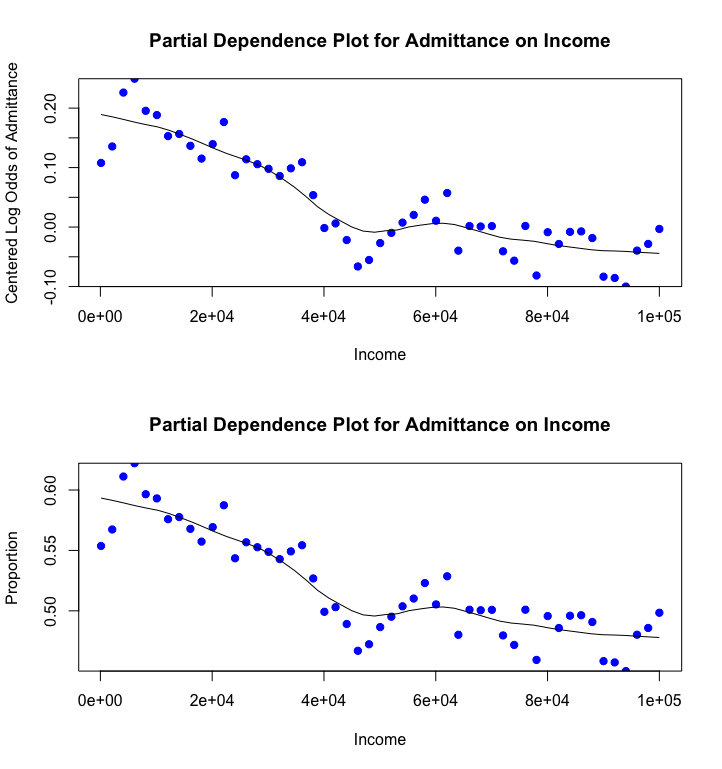
\includegraphics[scale=.60]{DEPENDENCE5}
\caption{Partial Dependence Plots for Income}
\end{figure}

\begin{figure} [h]
\centering
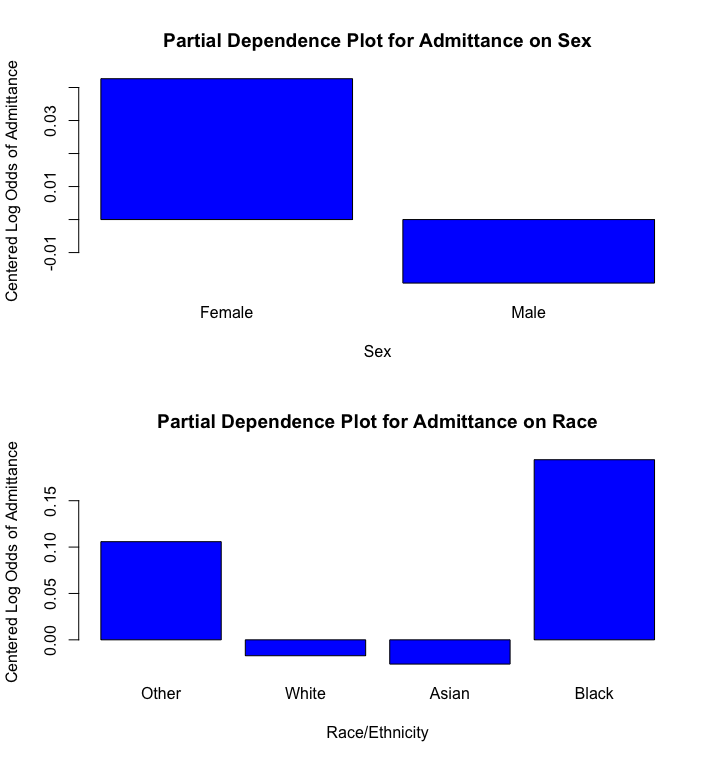
\includegraphics[scale=.60]{DEPENDENCE1}
\caption{Partial Dependence Plots for Sex and Race/Ethnicity}
\end{figure}

\end{document}  